\section{Runtime Interface and Evaluation Integration}
\label{sec:runtime-interface}

The user interface is not treated as a primary research contribution of this thesis. It is a supporting layer that exposes the agent backend, human-confirmation flow, and evaluation runner during development. The main implementation focus remains the agent architecture, MCP tool layer, resettable mock states, dataset construction process, and trace-based evaluation.

\subsection{Interface Role in the System}

The implementation provides a lightweight React + Vite interface for sending natural-language requests to the FastAPI agent service. Its role is deliberately narrow:

\begin{itemize}
    \item submit user prompts to the OpenAI-compatible chat endpoint,
    \item display final answers and selected status events from the agent runtime,
    \item relay explicit confirm/cancel decisions for pending state-changing operations,
    \item expose trace information that is useful for debugging agent behavior.
\end{itemize}

The screenshots below are captured from a live session running the fine-tuned Qwen2.5-14B model with the trained QLoRA adapter (\texttt{DanhVuiVe/slurm-agent-qwen14b-lora-final}), demonstrating real agent behaviour produced by the fine-tuned model rather than a base or prompted baseline.

\begin{figure}[H]
    \centering
    \begin{subfigure}[b]{\textwidth}
        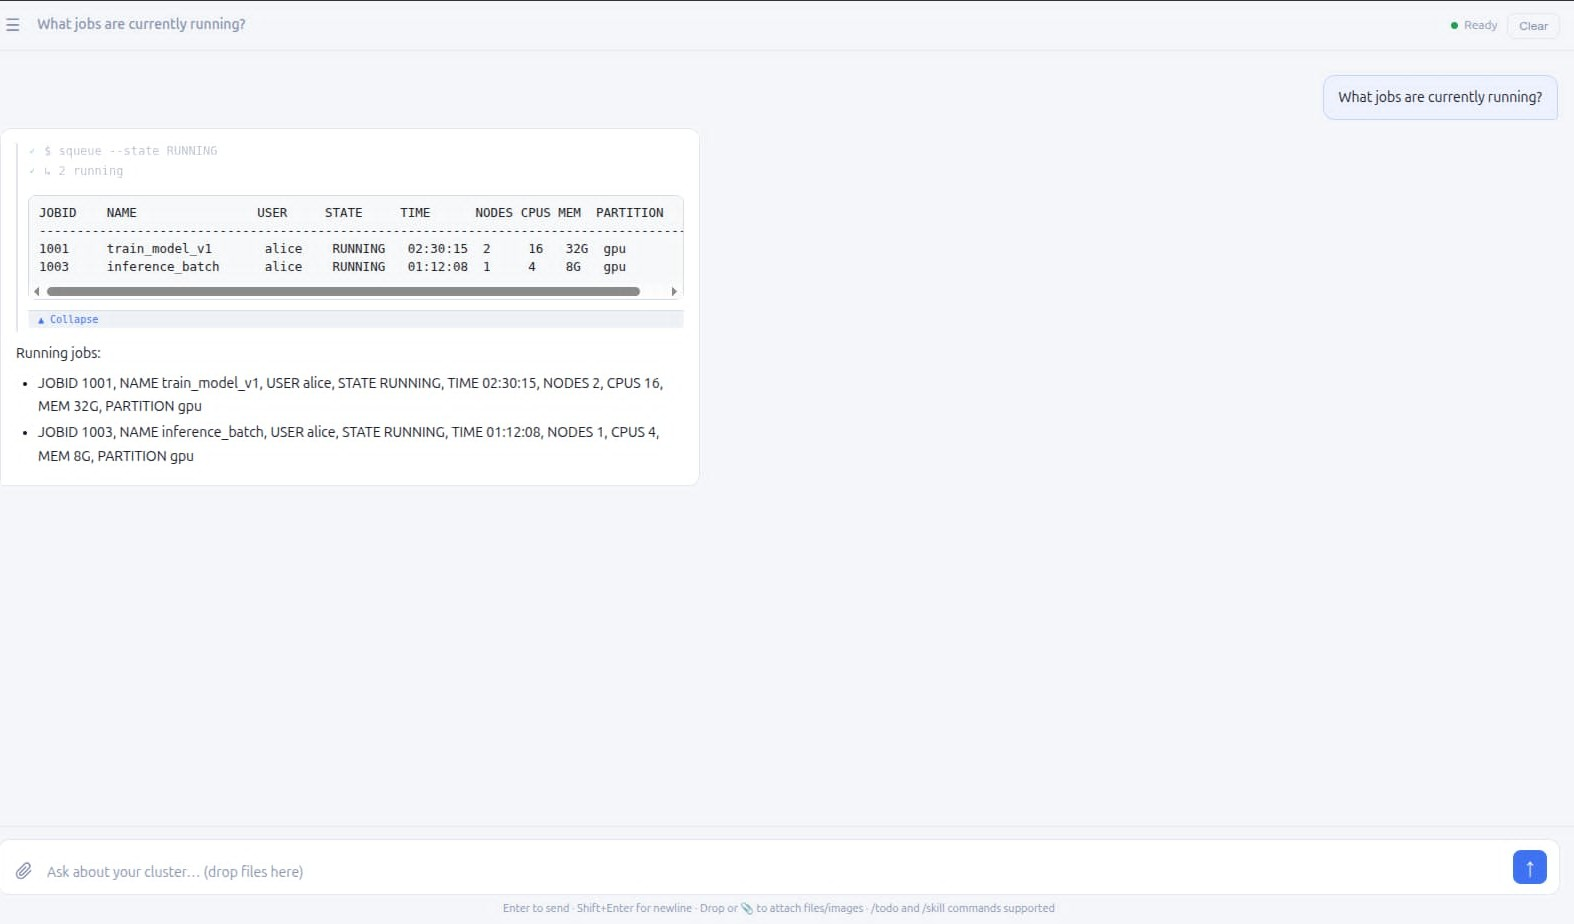
\includegraphics[width=\textwidth,height=0.27\textheight,keepaspectratio]{images/UI_before_HITL.jpg}
        \caption{The user asks ``What jobs are currently running?'' The fine-tuned LoRA model translates the query into an \texttt{squeue} call and renders the result as a table plus bulleted breakdown, showing two active jobs (\texttt{train\_model\_v1} and \texttt{inference\_batch}) for user \texttt{alice} with GPU resource details.}
        \label{fig:ui-before-hitl}
    \end{subfigure}
    \vspace{0.5em}

    \begin{subfigure}[b]{\textwidth}
        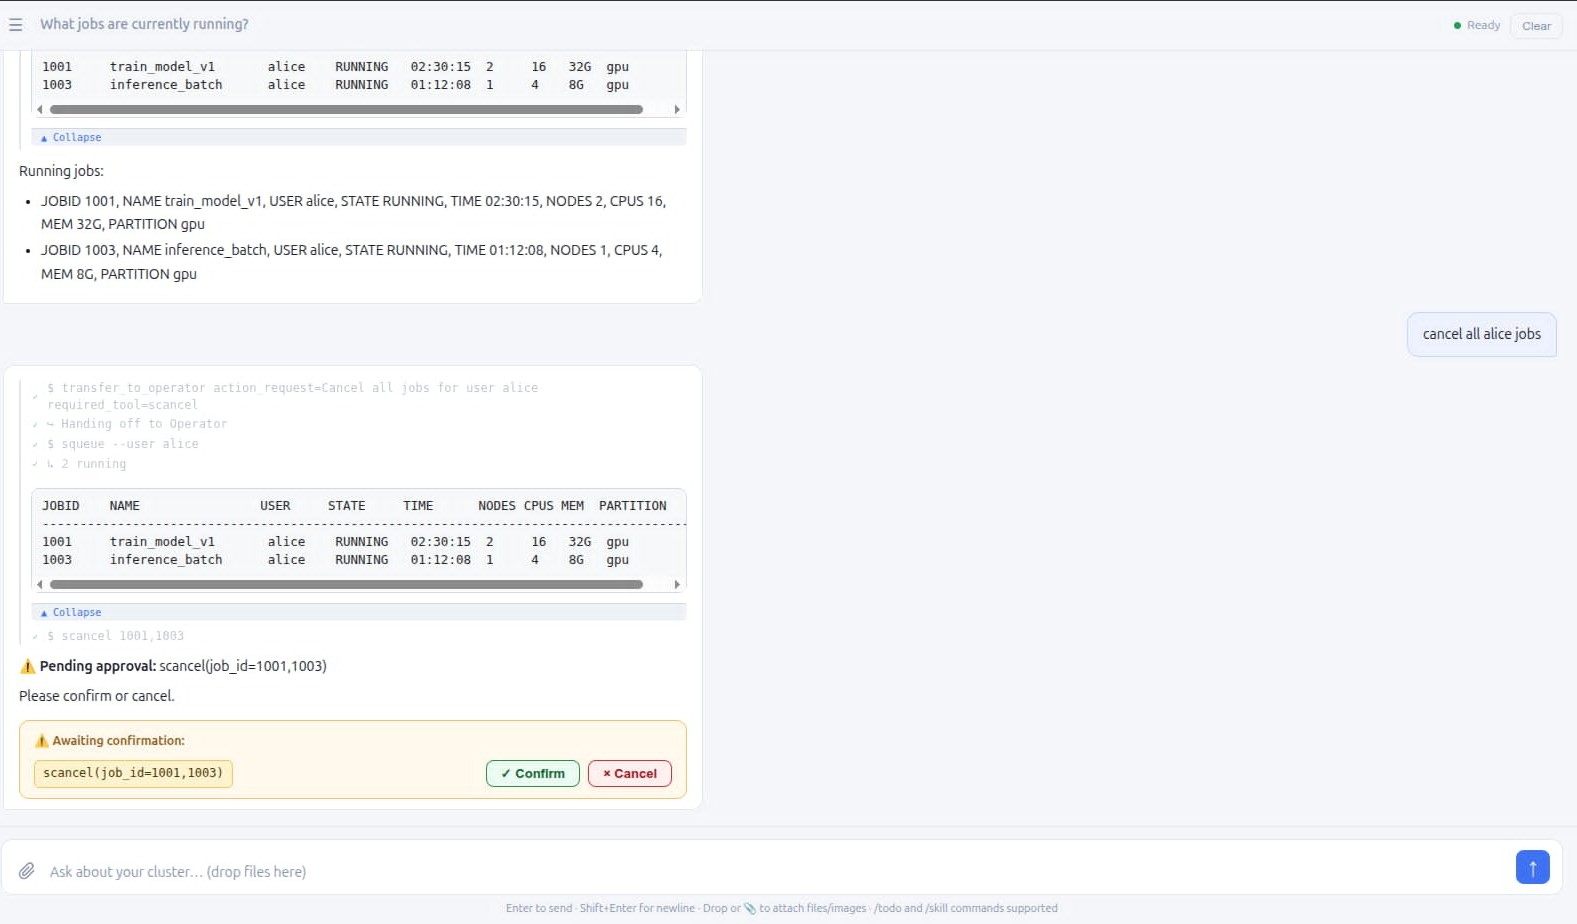
\includegraphics[width=\textwidth,height=0.27\textheight,keepaspectratio]{images/UI_during_HITL.jpg}
        \caption{The user issues ``cancel all alice jobs.'' Because \texttt{scancel} is destructive, the HITL safety layer intercepts execution and presents the exact call---\texttt{scancel(job\_id=1001,1003)}---with explicit \textit{Confirm} and \textit{Cancel} buttons, requiring a manual decision before any state change.}
        \label{fig:ui-during-hitl}
    \end{subfigure}
    \vspace{0.5em}

    \begin{subfigure}[b]{\textwidth}
        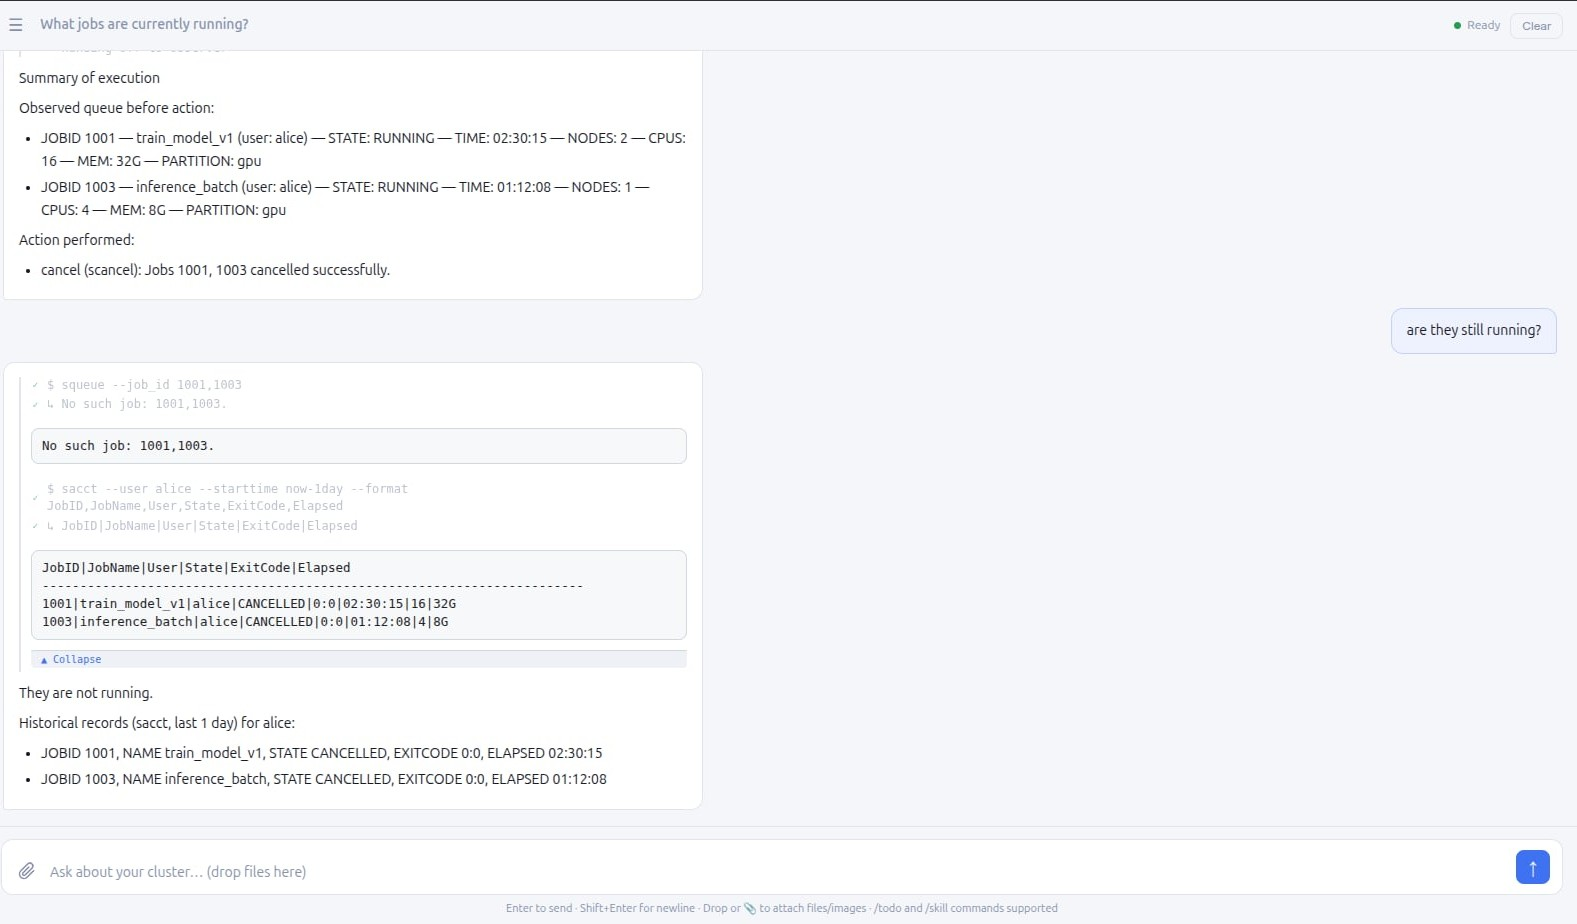
\includegraphics[width=\textwidth,height=0.27\textheight,keepaspectratio]{images/UI_after_HITL.jpg}
        \caption{After confirmation, \texttt{scancel} executes for job IDs 1001 and 1003. A follow-up \texttt{squeue} returns ``No such job'' for both, and the historical table shows \texttt{CANCELLED} state with exit codes and elapsed time, providing a full audit trail.}
        \label{fig:ui-after-hitl}
    \end{subfigure}
    \caption{End-to-end Human-in-the-Loop (HITL) confirmation flow, powered by the fine-tuned QLoRA model. Top: read-only cluster query; Middle: destructive action intercepted for manual approval; Bottom: post-execution verification of the cancelled jobs.}
    \label{fig:frontend-hitl-flow}
\end{figure}

This interface makes manual testing convenient, but the architectural boundary is the backend API.

\subsection{Agent Service API}

The agent service is implemented in \texttt{agent/main.py}. It exposes an OpenAI-compatible \texttt{/v1/chat/completions} endpoint that receives the user request, initializes or resumes the session, routes the request through the multi-agent backend, and streams structured events back to the caller. The event stream is mainly an implementation mechanism for carrying status updates, tool outputs, pending actions, final answer text, and evaluation traces.

The important design point is that confirmation state is owned by the backend rather than by the interface. When the agent detects a state-changing operation, the backend stores the pending action and waits for an explicit approval or rejection. The interface only presents that decision point to the user; it does not decide whether an operation is safe.

\subsection{Evaluation Integration}

The evaluation path uses the same backend behavior as manual interaction. The evaluator loads cases from \texttt{evaluation/dataset.json}, resets the mock Slurm state to the case's \texttt{source\_state}, submits the prompt to the live agent endpoint, records observed tools and handoffs, applies HITL decisions when required, and scores the result against ground truth labels.

An auxiliary evaluation backend provides controls for running single cases, running the full benchmark, stopping a run, and exporting result artifacts. An optional inspection view can display these artifacts, but the thesis treats the artifact itself as the evidence: dataset row, source state, target state, expected tools, observed tools, routing behavior, HITL behavior, response evidence, and state score.

